% $Id$

The \LinearPDE class is used to define a general linear, steady, second order PDE
for an unknown function $u$ on a given $\Omega$ defined through a \Domain object.
In the following $\Gamma$ denotes the boundary of the domain $\Omega$. $n$ denotes
the outer normal field on $\Gamma$. 

For a single PDE with a solution with a single component the linear PDE is defined in the 
following form:
\begin{equation}\label{LINEARPDE.SINGLE.1}
-(A\hackscore{jl} u\hackscore{,l}){,j}+(B\hackscore{j} u)\hackscore{,j}+C\hackscore{l} u\hackscore{,l}+D u =-X\hackscore{j,j}+Y \; .
\end{equation}
$u_{,j}$ denotes the derivative of $u$ with respect to the $j$-th spatial direction. Einstein's summation convention, ie. summation over indexes appearing twice in a term of a sum is performed, is used. 
The coefficients $A$, $B$, $C$, $D$, $X$ and $Y$ have to be specified through \Data objects in the 
\Function on the PDE or objects that can be converted into such \Data objects. 
$A$ is a \RankTwo, $B$, $C$ and $X$ are \RankOne and $D$ and $Y$ are scalar. 
The following natural
boundary conditions are considered \index{boundary condition!natural} on $\Gamma$:
\begin{equation}\label{LINEARPDE.SINGLE.2}
n\hackscore{j}(A\hackscore{jl} u\hackscore{,l}+B\hackscore{j} u)+d u=n\hackscore{j}X\hackscore{j} + y  \;.
\end{equation}
Notice that the coefficients $A$, $B$ and $X$ are defined in the PDE. The coefficients $d$ and $y$ are  
each a \Scalar in the \FunctionOnBoundary.  Constraints \index{constraint} for the solution prescribing the value of the 
solution at certain locations in the domain. They have the form
\begin{equation}\label{LINEARPDE.SINGLE.3}
u=r \mbox{ where } q>0
\end{equation}
$r$ and $q$ are each \Scalar where $q$ is the characteristic function
\index{characteristic function} defining where the constraint is applied.
The constraints defined by \eqn{LINEARPDE.SINGLE.3} override any other condition set by \eqn{LINEARPDE.SINGLE.1}
or \eqn{LINEARPDE.SINGLE.2}. The PDE is symmetrical \index{symmetrical} if
\begin{equation}\label{LINEARPDE.SINGLE.4}
A\hackscore{jl}=A\hackscore{lj} \mbox{ and } B\hackscore{j}=C\hackscore{j}
\end{equation}
For a system of PDEs and a solution with several components the PDE has the form
\begin{equation}\label{LINEARPDE.SYSTEM.1}
-(A\hackscore{ijkl} u\hackscore{k,l}){,j}+(B\hackscore{ijk} u_k)\hackscore{,j}+C\hackscore{ikl} u\hackscore{k,l}+D\hackscore{ik} u_k =-X\hackscore{ij,j}+Y\hackscore{i} \; .
\end{equation}
$A$ is a \RankFour, $B$ and $C$ are each a \RankThree, $D$ and $X$ are each a \RankTwo and $Y$ is a \RankOne. 
The natural boundary conditions \index{boundary condition!natural} take the form:
\begin{equation}\label{LINEARPDE.SYSTEM.2}
n\hackscore{j}(A\hackscore{ijkl} u\hackscore{k,l}){,j}+(B\hackscore{ijk} u_k)+d\hackscore{ik} u_k=n\hackscore{j}-X\hackscore{ij}+y\hackscore{i}  \;.
\end{equation}
The coefficient $d$ is a \RankTwo and $y$ is a  
\RankOne both in the \FunctionOnBoundary. Constraints \index{constraint} take the form
\begin{equation}\label{LINEARPDE.SYSTEM.3}
u\hackscore{i}=r\hackscore{i} \mbox{ where } q\hackscore{i}>0
\end{equation}
$r$ and $q$ are each \RankOne. Notice that at some locations not necessarily all components must 
have a constraint. The system of PDEs is symmetrical \index{symmetrical} if
\begin{eqnarray}\label{LINEARPDE.SYSTEM.4}
A\hackscore{ijkl}=A\hackscore{klij} \\
B\hackscore{ijk}=C\hackscore{kij} \\
D\hackscore{ik}=D\hackscore{ki} \\
d\hackscore{ik}=d\hackscore{ki} \
\end{eqnarray}
\LinearPDE also supports solution discontinuities \index{discontinuity} over contact region $\Gamma^{contact}$
in the domain $\Omega$. To specify the conditions across the discontinuity we are using the
generalised flux $J$ which is in the case of a systems of PDEs and several components of the solution
defined as 
\begin{equation}\label{LINEARPDE.SYSTEM.5}
J\hackscore{ij}=A\hackscore{ijkl}u\hackscore{k,l}+B\hackscore{ijk}u\hackscore{k}-X\hackscore{ij}
\end{equation}
For the case of single solution component and single PDE $J$ is defined
\begin{equation}\label{LINEARPDE.SINGLE.5}
J\hackscore{j}=A\hackscore{jl}u\hackscore{,l}+B\hackscore{j}u\hackscore{k}-X\hackscore{j}
\end{equation}
In the context of discontinuities \index{discontinuity} $n$ denotes the normal on the 
discontinuity pointing from side 0 towards side 1. For a system of PDEs
the contact condition takes the form
\begin{equation}\label{LINEARPDE.SYSTEM.6}
n\hackscore{j} J^{0}\hackscore{ij}=n\hackscore{j} J^{1}\hackscore{ij}=y^{contact}\hackscore{i} - d^{contact}\hackscore{ik} [u]\hackscore{k} \; .
\end{equation}
where $J^{0}$ and $J^{1}$ are the fluxes on side $0$ and side $1$ of the
discontinuity $\Gamma^{contact}$, respectively. $[u]$, which is the difference
of the solution at side 1 and at side 0, denotes the jump of $u$ across $\Gamma^{contact}$.
The coefficient $d^{contact}$ is a \RankTwo and $y^{contact}$ is a  
\RankOne both in the \FunctionOnContactZero or \FunctionOnContactOne.
In case of a single PDE and a single component solution the contact condition takes the form
\begin{equation}\label{LINEARPDE.SINGLE.6}
n\hackscore{j} J^{0}\hackscore{j}=n\hackscore{j} J^{1}\hackscore{j}=y^{contact} - d^{contact}[u]
\end{equation}
In this case the the coefficient $d^{contact}$ and $y^{contact}$ are eaach \Scalar
both in the \FunctionOnContactZero or \FunctionOnContactOne.
======================


We have used a special case of the \LinearPDE class, namely the
\Poisson class already in \Chap{FirstSteps}. 
Here we will write our own specialized sub-class of the \LinearPDE to define the Helmholtz equation
and use the \method{getSolution} method of parent class to actually solve the problem.

The form of a single PDE that can be handled by the \LinearPDE class is 
\begin{equation}\label{EQU.FEM.1}
-(A\hackscore{jl} u\hackscore{,l})\hackscore{,j}+D u =Y \; .
\end{equation}
We show here the terms which are relevant for the Helmholtz problem. 
The general form and systems is discussed in \Sec{SEC LinearPDE}.  
$A$, $D$ and $Y$ are the known coeffecients of the PDE. \index{partial differential equation!coefficients} 
Notice that $A$ is a matrix or tensor of order 2 and $D$ and $Y$ are scalar. 
They may be constant or may depend on their 
location in the domain but must not depend on the unknown solution $u$. 
The following natural boundary conditions \index{boundary condition!natural} that
are used in the \LinearPDE class have the form
\begin{equation}\label{EQU.FEM.2}
n\hackscore{j}A\hackscore{jl} u\hackscore{,l}+du=y  \;.
\end{equation}
where, as usual, $n$ denotes the outer normal field on the surface of the domain. Notice that 
the coefficient $A$ is already used in the PDE in \eqn{EQU.FEM.1}. $d$ and $y$ are given scalar coefficients.

By inspecting the Helmholtz equation \index{Helmholtz equation} 
we can easily assign values to the coefficients in the 
general PDE of the \LinearPDE class:
\begin{equation}\label{DIFFUSION HELM EQ 3}
\begin{array}{llllll}
A\hackscore{ij}=\kappa \delta\hackscore{ij} & D=\omega & Y=f \\
d=\eta & y= g &  \\
\end{array}
\end{equation}
$\delta\hackscore{ij}$ is the Kronecker symbol \index{Kronecker symbol} defined by $\delta\hackscore{ij}=1$ for
$i=j$ and $0$ otherwise.

We want to implement a 
new class which we will call \class{Helmholtz} that provides the same methods as the \LinearPDE class but
is described using the coefficients $\kappa$, $\omega$, $f$, $\eta$, 
$g$ rather than the general form given by \eqn{EQU.FEM.1}. 
Python's mechanism of subclasses allows us to do this in a very simple way.
The \Poisson class of the \linearPDEs module,
which we have already used in \Chap{FirstSteps}, is in fact a subclass of the more general
\LinearPDE class. That means that all methods (such as the \method{getSolution})
from the parent class \LinearPDE are available for any \Poisson object. However, new
methods can be added and methods of the parent class can be redefined. In fact,
the \Poisson class redefines the \method{setValue} of the \LinearPDE class which is called to assign 
values to the coefficients of the PDE. This is exactly what we will do when we define 
our new \class{Helmholtz} class:
\begin{python}
from esys.linearPDEs import LinearPDE
import numarray
class Helmholtz(LinearPDE):
   def setValue(self,kappa=0,omega=1,f=0,eta=0,g=0)
        ndim=self.getDim()
        kronecker=numarray.identity(ndim)
        self.setValue(A=kappa*kronecker,D=omega,Y=f,d=eta,y=g)
\end{python}
\code{class Helmholtz(linearPDE)} declares the new \class{Helmholtz} class as a subclass 
of \LinearPDE which we have imported in the first line of the script. 
We add the method \method{setValue} to the class which overwrites the 
\method{setValue} method of the \LinearPDE class. The new method which has the 
parameters of the Helmholtz \eqn{DIFFUSION HELM EQ 1} as arguments 
maps the parameters of the coefficients of the general PDE defined 
in \eqn{EQU.FEM.1}. We are actually using the \method{_LinearPDE__setValue} of 
the \LinearPDE class. 
The coefficient \var{A} involves the Kronecker symbol. We use the
\numarray function \function{identity} which returns a square matrix with ones on the
main diagonal and zeros off the main diagonal. The argument of \function{identity} gives the order of the matrix.
The \method{getDim} of the \LinearPDE class object \var{self} to get the spatial dimensions of the domain of the
PDE. As we will make use of the \class{Helmholtz} class several times, it is convenient to 
put its definition into a file which we name \file{mytools.py} available in the \ExampleDirectory.
You can use your favourite editor to create and edit the file.   

An object of the \class{Helmholtz} class is created through the statments:
\begin{python}
from mytools import Helmholtz
mypde = Helmholtz(mydomain)
mypde.setValue(kappa=10.,omega=0.1,f=12)
u = mypde.getSolution()
\end{python}
In the first statement we import all definition from the \file{mytools.py} \index{scripts!\file{mytools.py}}. Make sure
that \file{mytools.py} is in the directory from where you started Python.
\var{mydomain} is the \Domain of the PDE which we have undefined here. In the third statment values are
assigned to the PDE parameters. As no values for arguments \var{eta} and \var{g} are
specified, the default values $0$ are used. \footnote{It would be better to use the default value 
\var{escript.Data()} rather then $0$ as then the coefficient would be defined as being not present and
would not be processed when the PDE is evaluated}. In the fourth statement the solution of the
PDE is returned. 

To test our \class{Helmholtz} class on a rectangular domain
of length $l\hackscore{0}=5$ and height $l\hackscore{1}=1$, we choose a simple test solution. Actually, we 
we take $u=x\hackscore{0}$ and then calculate the right hand side terms $f$ and $g$ such that
the test solution becomes the solution of the problem. If we assume $\kappa$ as being constant, 
an easy calculation shows that we have to choose $f=\omega \cdot x\hackscore{0}$. On the boundary we get
$\kappa n\hackscore{i} u\hackscore{,i}=\kappa n\hackscore{0}$.  
So we have to set $g=\kappa n\hackscore{0}+\eta x\hackscore{0}$. The following script \file{helmholtztest.py} 
\index{scripts!\file{helmholtztest.py}} which is available in the \ExampleDirectory
implements this test problem using the \finley PDE solver:
\begin{python}
from mytools import Helmholtz
from esys.escript import Lsup
from esys.finley import Rectangle
#... set some parameters ...
kappa=1.
omega=0.1
eta=10.
#... generate domain ...
mydomain = Rectangle(l0=5.,l1=1.,n0=50, n1=10)
#... open PDE and set coefficients ...
mypde=Helmholtz(mydomain)
n=mydomain.getNormal()
x=mydomain.getX()
mypde.setValue(kappa,omega,omega*x[0],eta,kappa*n[0]+eta*x[0])
#... calculate error of the PDE solution ...
u=mypde.getSolution()
print "error is ",Lsup(u-x[0])
\end{python}
The script is similar to the script \file{mypoisson.py} dicussed in \Chap{FirstSteps}.
\code{mydomain.getNormal()} returns the outer normal field on the surface of the domain. The function \function{Lsup}
is imported by the \code{from esys.escript import Lsup} statement and returns the maximum absulute value of its argument. 
The error shown by the print statement should be in the order of $10^{-7}$. As piecewise bi-linear interpolation is
used to approximate the solution and our solution is a linear function of the spatial coordinates one might 
expect that the error would be zero or in the order of machine precision (typically $\approx 10^{-15}$). 
However most PDE packages use an iterative solver which is terminated
when a given tolerance has been reached. The default tolerance is $10^{-8}$. This value can be altered by using the 
\method{setTolerance} of the \LinearPDE class. 

\subsection{The Transition Problem}
\label{DIFFUSION TRANS SEC}
Now we are ready to solve the original time dependent problem. The main 
part of the script is the loop over time $t$ which takes the following form:
\begin{python}
t=0
T=Tref
mypde=Helmholtz(mydomain)
while t<t_end:
      mypde.setValue(kappa,rhocp/h,q+rhocp/h*T,eta,eta*Tref)
      T=mypde.getSolution()
      t+=h
\end{python}
\var{kappa}, \var{rhocp}, \var{eta} and \var{Tref} are input parameters of the model. \var{q} is the heat source
in the domain and \var{h} is the time step size. Notice that the \class{Hemholtz} class object \var{mypde}
is created before the loop over time is entered while in each time step only the coefficients
are reset in each time step. This way some information about the representation of the PDE can be reused 
\footnote{The efficience can be improved further by setting the coefficients in the operator
\var{kappa}, \var{omega} and \var{eta} before entering the \code{while}-loop and only updating the coefficients
in the right hand side \var{f} and \var{g}. This needs a more careful implementation of the \method{setValue}
method but gives the advantage that the \LinearPDE class can save rebuilding the PDE operator.}. The variable \var{T}
holds the current temperature. It is used to calculate the right hand side coefficient \var{f} in the
Helmholtz equation in \eqn{DIFFUSION HELM EQ 1}. The statement \code{T=mypde.getSolution()} overwrites \var{T} with the 
temperature of the new time step $\var{t}+\var{h}$. To get this iterative process going we need to specify the
initial temperature distribution, which equal to $T\hackscore{ref}$.

The heat source \var{q} which is defined in \eqn{DIFFUSION TEMP EQ 1b} is \var{qc}
in an area defined as a circle of radius \var{r} and center \var{xc} and zero outside this circle.
\var{q0} is a fixed constant. The following script defines \var{q} as desired:  
\begin{python}
from esys.escript import length
xc=[0.02,0.002]
r=0.001
x=mydomain.getX()
q=q0*(length(x-xc)-r).whereNegative()
\end{python}
\var{x} is a \Data class object of
the \escript module defining locations in the \Domain \var{mydomain}.
The \function{length()} imported from the \escript module returns the 
Euclidean norm:
\begin{equation}\label{DIFFUSION HELM EQ 3aba}
\|y\|=\sqrt{
y\hackscore{i}
y\hackscore{i}
} = \function{esys.escript.length}(y)
\end{equation}
So \code{length(x-xc)} calculates the distances  
of the location \var{x} to the center of the circle \var{xc} where the heat source is acting.
Note that the coordinates of \var{xc} are defined as a list of floating point numbers. It is independently
converted into a \Data class object before being subtracted from \var{x}. The method \method{whereNegative} of
a \Data class object, in this case the result of the expression 
\code{length(x-xc)-r}, returns a \Data class which is equal to one where the object is negative and
zero elsewhere. After multiplication with \var{qc} we get a function with the desired property.

Now we can put the components together to create the script \file{diffusion.py} which is available in the \ExampleDirectory:
\index{scripts!\file{diffusion.py}}:
\begin{python}
from mytools import Helmholtz
from esys.escript import Lsup
from esys.finley import Rectangle
#... set some parameters ...
xc=[0.02,0.002]
r=0.001
qc=50.e6
Tref=0.
rhocp=2.6e6
eta=75.
kappa=240.
tend=5.
# ... time, time step size and counter ...
t=0
h=0.1
i=0
#... generate domain ...
mydomain = Rectangle(l0=0.05,l1=0.01,n0=250, n1=50)
#... open PDE ...
mypde=Helmholtz(mydomain)
# ... set heat source: ....
x=mydomain.getX()
q=qc*(length(x-xc)-r).whereNegative()
# ... set initial temperature ....
T=Tref
# ... start iteration:
while t<tend:
      i+=1
      t+=h
      print "time step :",t
      mypde.setValue(kappa=kappa,omega=rhocp/h,f=q+rhocp/h*T,eta=eta,g=eta*Tref)
      T=mypde.getSolution()
      T.saveDX("T%d.dx"%i)
\end{python}
The script will create the files \file{T.1.dx},
 \file{T.2.dx}, $\ldots$, \file{T.50.dx} in the directory where the script has been started. The files give the 
temperature distributions at time steps $1$, $2$, $\ldots$, $50$ in the \OpenDX file format. 

\begin{figure}
\centerline{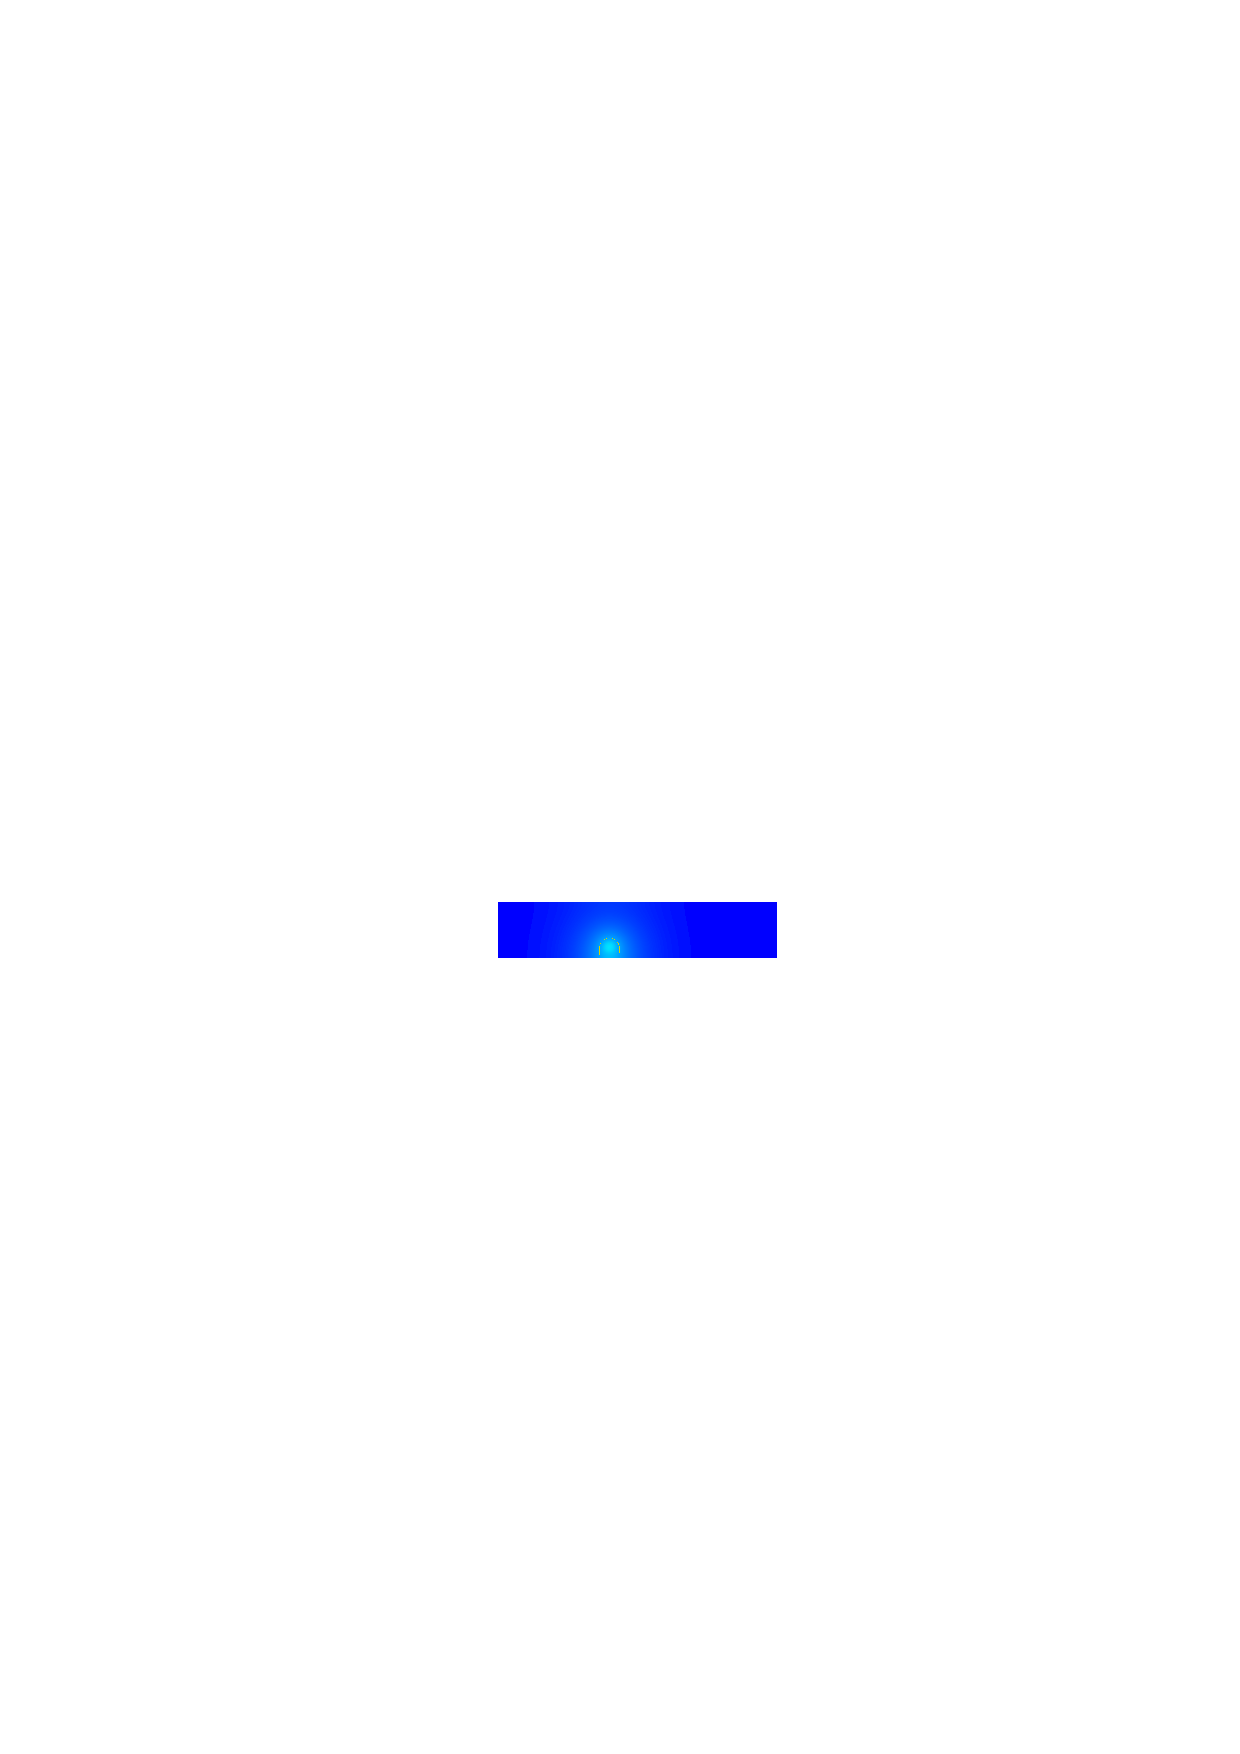
\includegraphics[width=\figwidth]{DiffusionRes1}}
\centerline{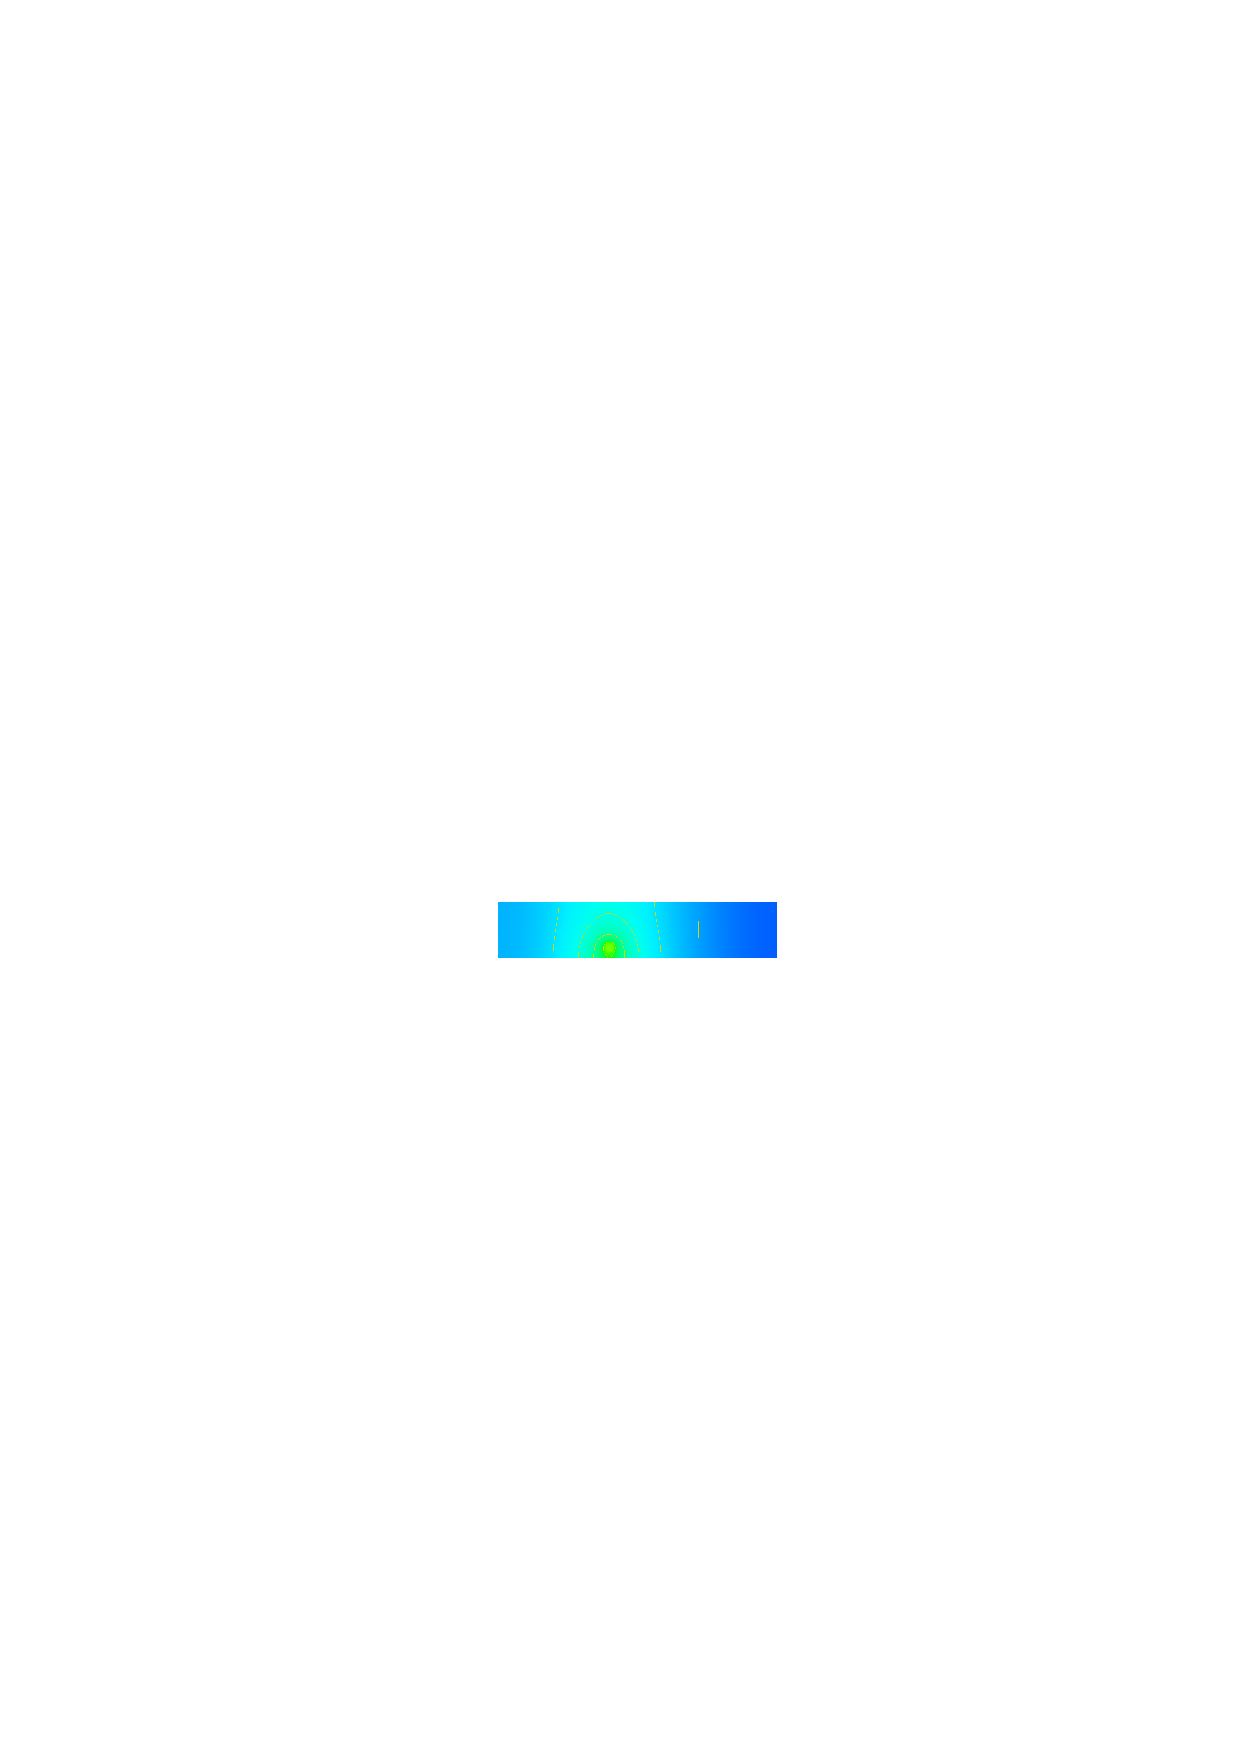
\includegraphics[width=\figwidth]{DiffusionRes16}}
\centerline{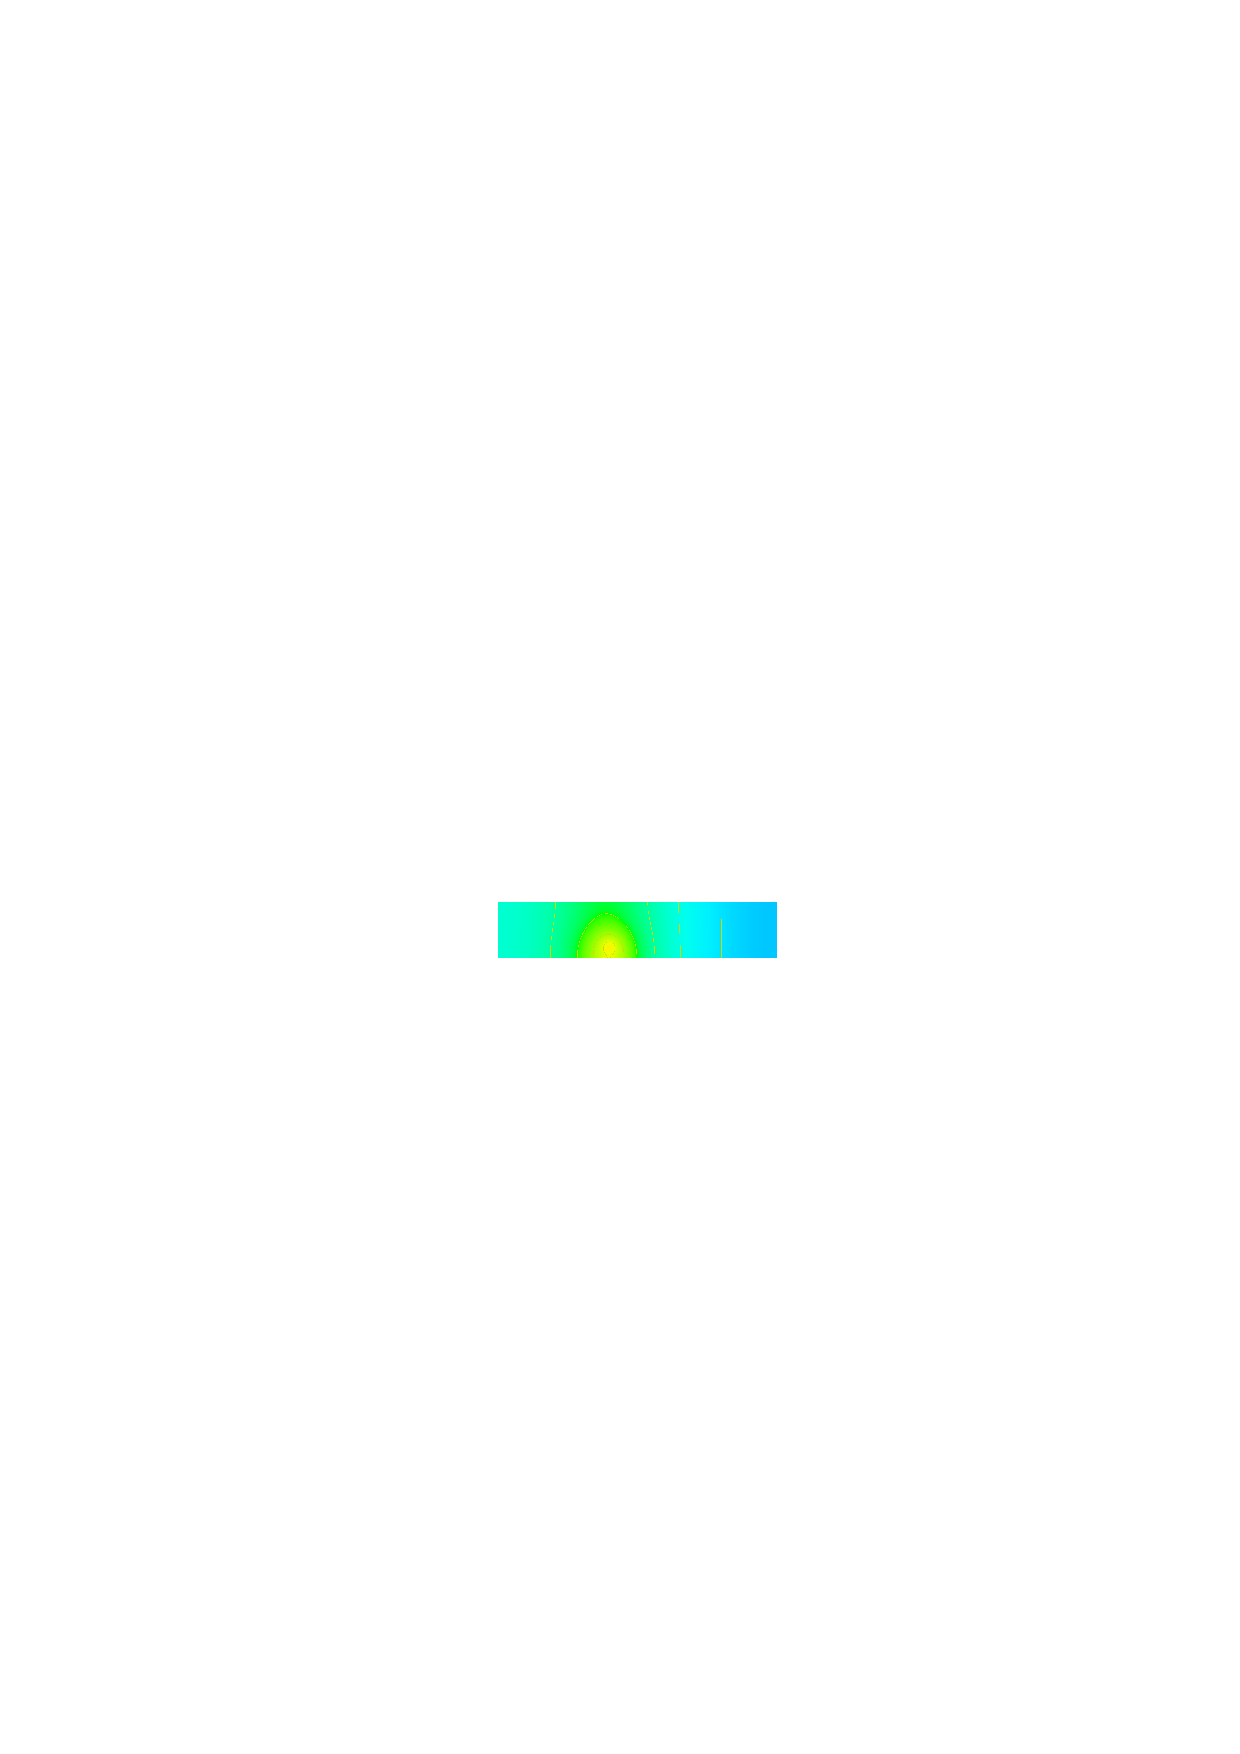
\includegraphics[width=\figwidth]{DiffusionRes32}}
\centerline{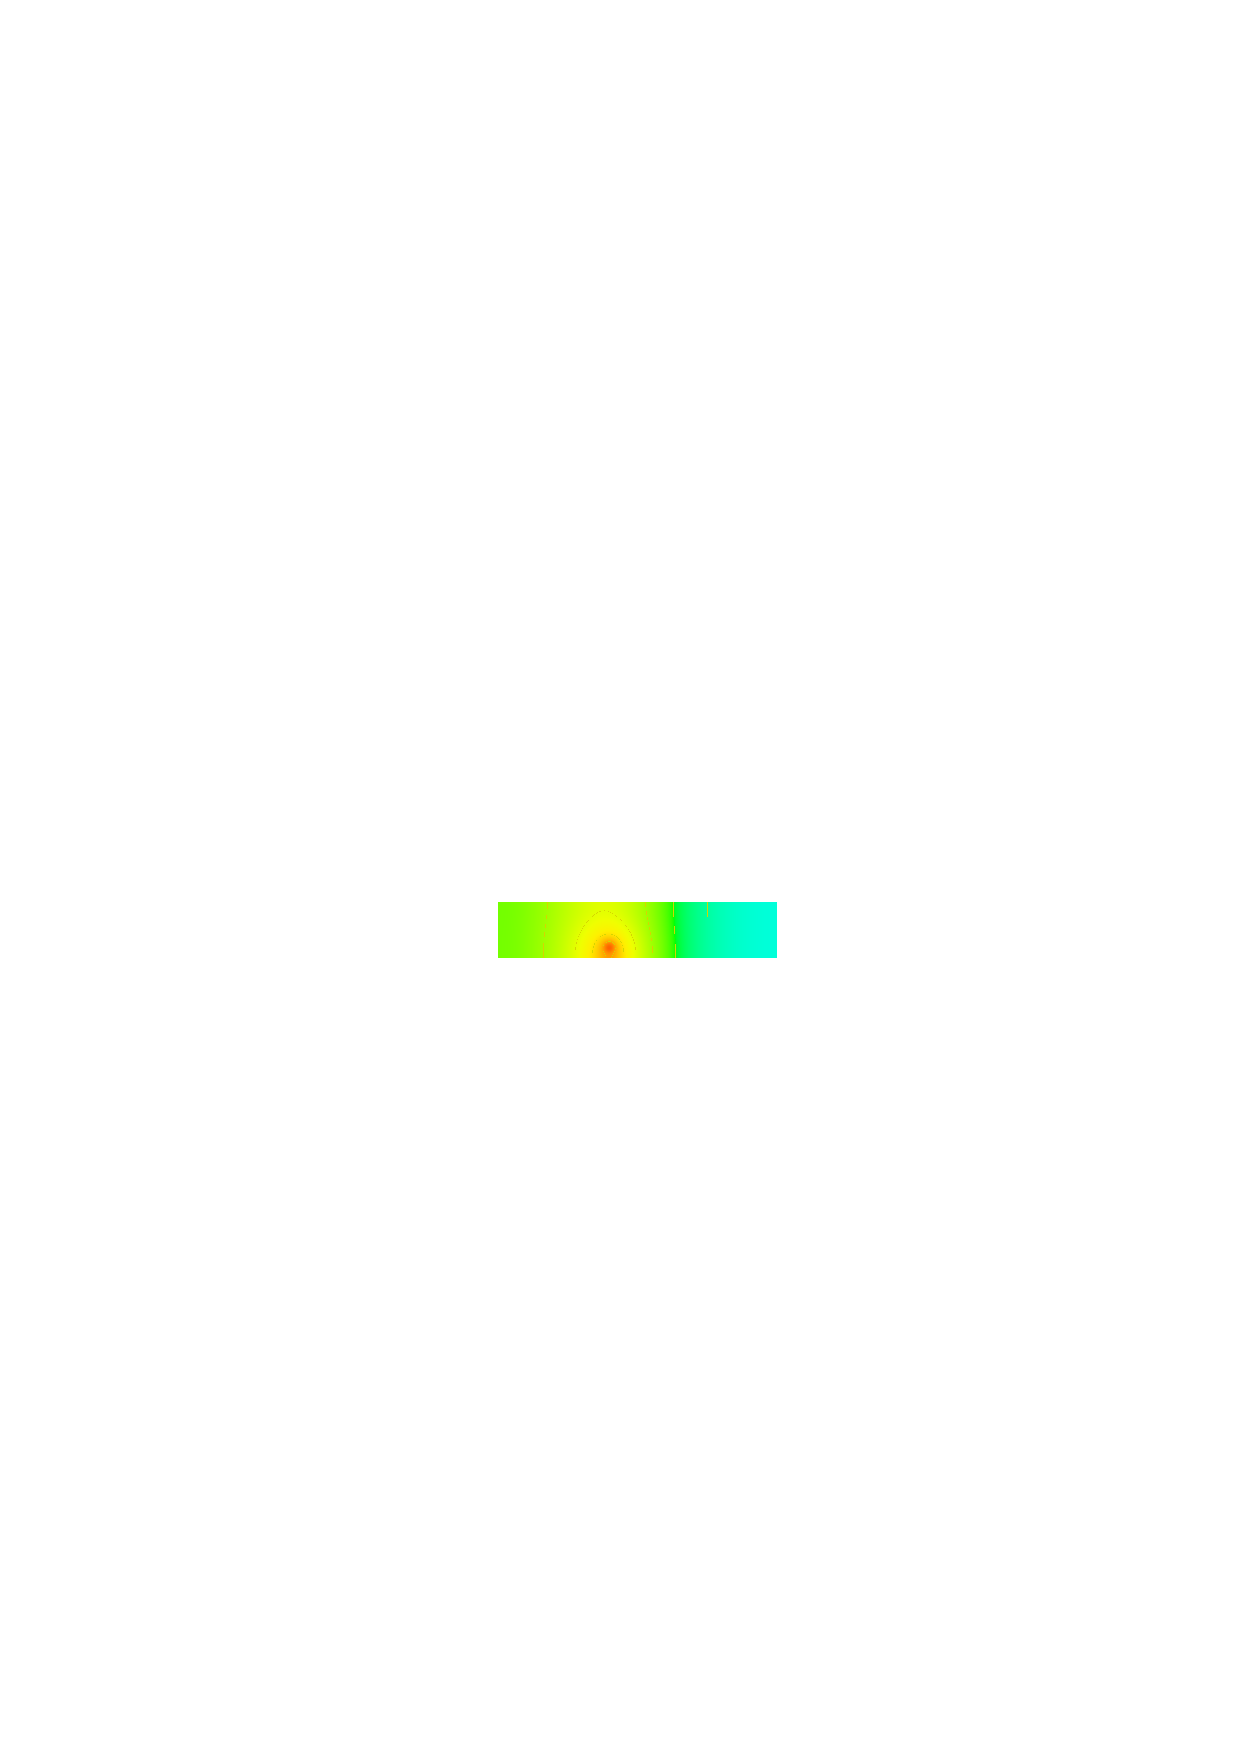
\includegraphics[width=\figwidth]{DiffusionRes48}}
\caption{Results of the Temperture Diffusion Problem for Time Steps $1$ $16$, $32$ and $48$.}
\label{DIFFUSION FIG 2}
\end{figure}

An easy way to visualize the results is the command
\begin{verbatim}
dx -edit diffusion.net &
\end{verbatim}
where \file{diffusion.net} is an \OpenDX script available in the \ExampleDirectory.
Use the \texttt{Sequencer} to move forward and and backwards in time. 
\fig{DIFFUSION FIG 2} shows the result for some selected time steps.
====
\section{Bending Beam under Uniform Load}
\label{BEAM CHAP}
\sectionauthor{Jannine Eisenmann}{}

Given is a two-dimension bending beam which is fixed in all directions
at the left end and free at the other, see \fig{BEAM FIG 1}. Furthermore the beam is loaded
with a uniform load $p$.

\begin{figure}
% \centerline{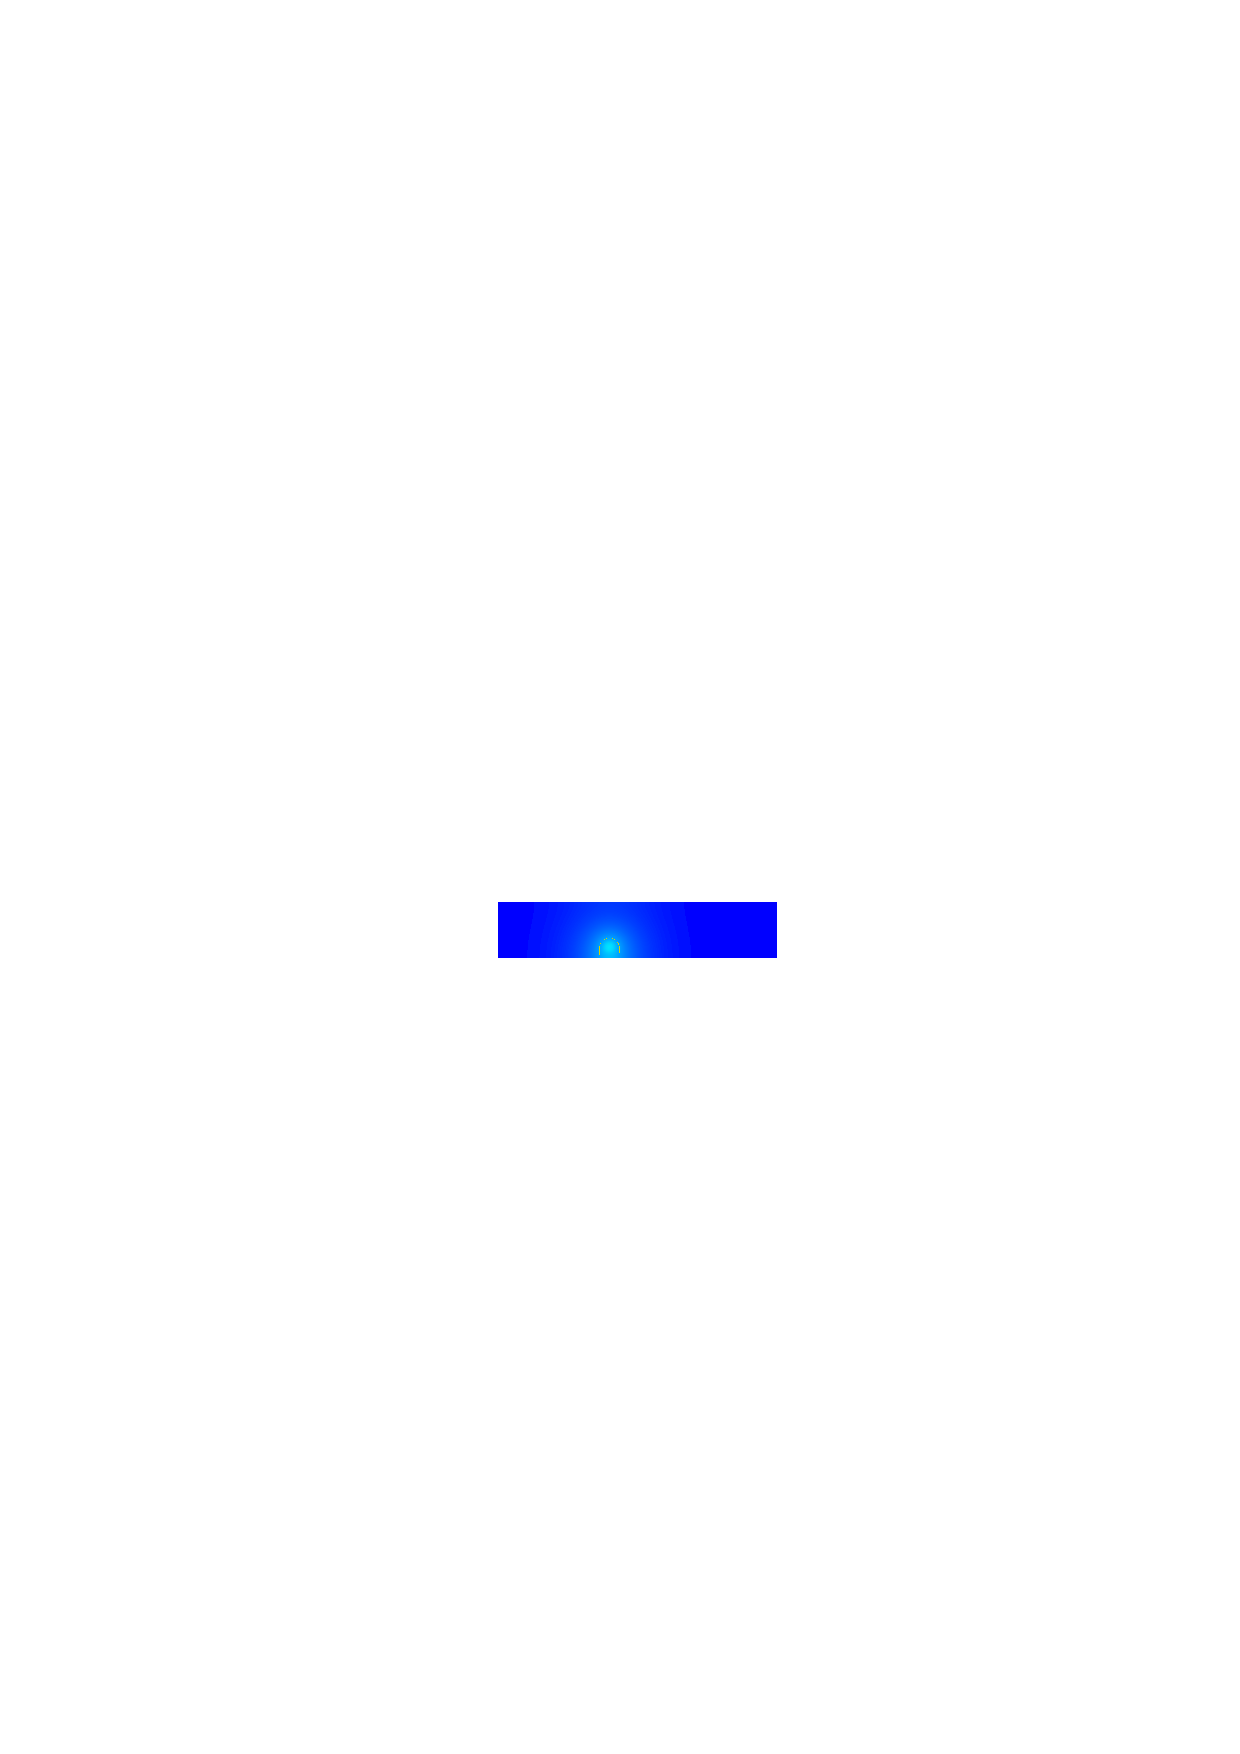
\includegraphics[width=\figwidth]{DiffusionRes1}}
\caption{Loaded Beam.}
\label{BEAM FIG 1}
\end{figure}



For emphasizing the displacement this picture is drawn (uebertrieben),
cause since we use the linear theory otherwise no displacements would
be visible. 
There are two ways of solving this problem: on the one hand one can
use the differential equation for the deformed neutral fibre of the
beam. This classical differential equation is based on several simplifying
assumptions concerning the statics and kinematics of the problem.
However the results are known to be highly accurate at least for slender
beams with length to hight ratios $> 10$. Alternatively, in connection
with finite element based differential equation toolkits one may simply
consider the beam as a special case of a 2D or 3D elastic continuum
problem and solve the stress equilibrium equations combined with Hooke's
law for the specific boundary conditions of a beam. Both cases assume
isotropic and linear elastic material properties.

The beam equation is easily solved analytically. The analytical solutions
can be used for benchmarkung finite element solutions. In section
1.2 we formluate a finite element code for general isotropic elasticity
problems including thin and deep beams under arbitrary loading conditiond
in 2D or 3D. 


\section{2-dimensional}
As the stress equilibrium equation is a partial differential equation
(PDE), we choose to use Finley to solve it, since Finley is a finite
element kernel library, that has been incorporated as a differential
equation solver into the python based numerical toolkit called escript.
We divided the beam into ten square elements of the size 1x1. Each
element consists of 8 nodes, which leads to a quadratic interpolation
of the model point displacements \\

The key ingredients is \textbf{Hooks Law}. We use Hooks Law because
we are dealing with \textbf{linear elastic material} \textbf{behaviour}.
We have \\


$\sigma_{ik}=2G\left(\varepsilon_{ik}+\frac{\nu}{1-2\nu}\cdot e\cdot\delta_{ik}\right)$\hfill{}(1)\\
where the engineering strain$\varepsilon_{ik}$is defined as:

$\varepsilon_{ik}=\frac{1}{2}\cdot\left(u_{k,i}+u_{i,k}\right)$\hfill{}(2)\\


with

\begin{enumerate}
\item e= Volume strain = $\varepsilon_{kk}$
\item $\delta_{ik}$= Kronecker symbol
\end{enumerate}
Inserting equation (2) in (1) (and with further mathematical conversions)
leads to the following partial differential equation :\\


$\sigma_{ij}=\left[\mu\left(\delta_{ik}\delta_{jl}+\delta_{il}\delta_{jk}\right)+\lambda\left(\delta_{ij}\delta_{kl}\right)\right]u_{k,l}$\\


For tension equilibrium we require:\\


$\sigma_{ij,j}=0$\\


which leads to the following expression:\\


\[
\left(\left[\mu\left(\delta_{ik}\delta_{jl}+\delta_{il}\delta_{jk}\right)+\lambda\left(\delta_{ij}\delta_{kl}\right)\right]u_{k,l}\right)_{,j}=0\]


with the natural boundary condition:

\[
n_{j}\sigma_{ij}=-p_{i}\]
\\
$p_{i}$ representing a uniform load on top of the beam.

A Dirichlet Boundary condition is assumed on the left end of the beam
for which no displacements can occure.\\
\\
\includegraphics[%
  width=0.60\linewidth,bb = 0 0 200 100, draft, type=eps]{/home/jeannine/sandbox/report/draws/dir_cond_beam.eps}\\
This is described in the code with the setting a mask for the left
end and setting values to that mask:

\begin{python}
q = xNodes{[}0{]}.whereZero(){*}{[}1.0,1.0{]}

r = Vector({[}0.0, 0.0{]}, where = nodes)
\end{python}
The Finley template PDE reads:\\


\[
-(A_{ijkl}u_{k,l})_{,j}-(B_{ijk}u_{k})_{,j}+C_{ikl}u_{k,l}+D_{ik}u_{k}=-X_{ij,j}+Y_{i}\]
\\
with the natural boundary condition:

\[
n_{j}(A_{ijkl}u_{k,l}+B_{ijkl}u_{k})+d_{ik}u_{k}=n_{j}X_{ij}+y_{i}on\Gamma_{i}^{D}\]


Yields by comparing the coefficients :

\begin{enumerate}
\item $A_{ijkl}$= $\left[\mu\left(\delta_{ik}\delta_{ij}+\delta_{jl}\delta_{il}\right)+\lambda\left(\delta_{ij}\delta_{kl}\right)\right]$
\item $y_{i}$= $-p_{i}$
\item $u_{k}$= displacement $u$
\end{enumerate}
$B_{ijk,}=C_{ikl}=D_{ik}=X_{ij}=Y_{i}=d_{ik}=0$\\


Where 0 in the last line is taken as a scalar, vector or tensor, depending
on what the belonging coefficient is.

These equations are the base for the \textbf{Finley Script}:

\begin{python}
from ESyS import {*}
import Finley



\#mu lamda

def mu (E, nu): \#= shear modul G

     return E/(2{*}(1+nu))

def lamda (E, nu):

     return (nu{*}E)/((1-2{*}nu){*}(1+nu))



def main()

     \#material, beam PROPERTIES

     L = 10.0         \#length of beam {[}m{]}

     h = 1            \#height of beam {[}m{]}

     p = 1            \#outer uniform load {[}kN/m{]}

     E0 = 210000      \#Young's modulus {[}kN/m\textasciicircum{}2{]}

     nu = 0.4         \#Poisson ratio {[}-{]}



     print \char`\"{}L=\char`\"{}, L

     print \char`\"{}h=\char`\"{}, h

     print \char`\"{}p=\char`\"{}, p

     print \char`\"{}E=\char`\"{}, E0

     print \char`\"{}nu=Poisson =\char`\"{}, nu

     print \char`\"{}mu=\char`\"{}, mu (E0,nu)

     print \char`\"{}lamda=\char`\"{}, lamda (E0,nu) 



     \#SET MESH for FE

     mesh= Finley.Rectangle(n0=10 ,n1=1 ,order=2, l0=L, l1=h)

     nodes = mesh.Nodes()

     xNodes = nodes.getX()

     elements = mesh.Elements()

     faceElements = mesh.FaceElements()

     xFaceElements = faceElements.getX()



     \#DISPLACEMENT boundary

     q = xNodes{[}0{]}.whereZero(){*}{[}1.,1.0{]}    \#setting the                                           mask for r

     r = Vector({[}0.0, 0.0{]}, where = nodes) \#fixed end



     \#STRESS boundary

     ymask = xFaceElements{[}1{]}.whereEqualTo(h)

     y = Vector({[}0, -p{]}, where = faceElements)

     y = y{*}ymask



     \#Finley coeff.

     A = Tensor4(0, where = elements)

     for i in range (2) :

        for j in range (2) :

           A{[}i,i,j,j{]}+= lamda (E0,nu)

           A{[}j,i,j,i{]}+= mu (E0,nu)

           A{[}j,i,i,j{]}+= mu (E0,nu)



     M,b = mesh.assemble(A=A, B=B, q=q,         

     y=y,r=r,type=CSR,num\_equations=2)

     u= M.iterative(b, tolerance=1e-8,iter\_max=50000,

     iterative\_method=PCG)

     print \char`\"{}u{[}0{]}=\char`\"{},u{[}0{]}

     print \char`\"{}u{[}1{]}=\char`\"{},u{[}1{]}

main()
\end{python}
The finer the mesh the more exact is the solution. E.g. a 20x2 mesh
is more exact than a 10x1 mesh. 

